\documentclass{article}
\linespread{1.3}
\usepackage[margin=50pt]{geometry}
\usepackage{amsmath, amsthm, amssymb, amsthm, tikz, fancyhdr, float, graphicx, spverbatim, systeme}
\pagestyle{fancy}
\renewcommand{\headrulewidth}{0pt}
\newcommand{\changefont}{\fontsize{15}{15}\selectfont}

\fancypagestyle{firstpageheader}{
  \fancyhead[R]{
    \changefont
    \parbox[t]{4cm}{
      Michael Huang\\
      EN.625.633.81\\
      Exam 2
    }
  }
}

\begin{document}

\thispagestyle{firstpageheader}
{\Large 

\section*{1.}

Using the Metropolis-Hastings Algorithm, we aim to simulate 10000 values of \(X\), where \(X \sim f_X(x)\) and \(f_X(x)  = \frac{8}{x^3}\) and \(x > 2\). \\ \\
We need to first choose a proposal distribution \(g(x_{t+1} | x_t)\). We want to pick a good candidate with respect to which we'll be calculating the acceptance probability 
\[
  \rho = \min(1, \frac{f_X(x_{t+1})g(x_t | x_{t+1})}{f_X(x_t) g(x_{t+1} | x_t)})
\]
We can use a normal distribution centered at \(x_t\) as our proposal distribution. Having symmetry in the distribution is an advantage in calculating the acceptance probability \(\rho\) above more easily, and also explores the distribution more uniformly than viable but asymmetric alternative proposals like an exponential, which would bias proposals and thus underexplore tails in our given exponential distribution. Something like the uniform distribution is also symmetrical, but requires figuring out good bounds, which is difficult since our \(x\) values are unbounded in the positive direction, and would lead to lower proposal acceptance rates in lower-density regions of the distribution. The normal distribution is ideal in proposing local moves that don't have these issues and also have appropriate step sizes. 
\begin{spverbatim}
> n = 10000
> 
> met_hastings = function(n, sd) {
+   x = rep(0, n)
+   acc = 0
+   j = 1
+   x[1] = 4
+   
+   while (j < n) {
+     # Propose candidate from normal distribution
+     x_cand = rnorm(1, mean = x[j], sd = sd)
+     
+     # Calculate acceptance probability
+     acc_prob = 0
+     if (x_cand > 2) {
+       acc_prob = min(1, (x[j] / x_cand)^3)
+     }
+     
+     # Decide whether to accept value 
+     acc_or_not = rbinom(1, 1, acc_prob)
+     
+     if (acc_or_not == 1) {
+       acc = acc + 1;
+       j = j + 1;
+       x[j] = x_cand
+     }
+     else {
+       j = j + 1
+       x[j] = x[j-1]
+     }	
+   }
+   
+   acc_probability = acc / n
+   print(paste("Acceptance probability:", acc_probability))
+   print(paste("Estimated mean:", mean(x)))
+   hist(x, breaks = 75, probability = TRUE,
+        main = paste("Metropolitan-Hastings Sample with sd =", sd))
+ }
> 
> met_hastings(n, 1)
[1] "Acceptance probability: 0.556"
[1] "Estimated mean: 3.47069848982251"
> met_hastings(n, 2)
[1] "Acceptance probability: 0.4264"
[1] "Estimated mean: 4.46785878128147"
> met_hastings(n, 4)
[1] "Acceptance probability: 0.2982"
[1] "Estimated mean: 4.97382948630564"
\end{spverbatim}
In this code, we run the Metropolis-Hastings algorithm to generate random numbers. We initialize a chain of numbers \(x\) which we'll generate step-by-step using the steps of the algorithm. We start at some arbitrary \(x\)-value. Then, within each step, we first use the proposal distribution of the normal distribution centered on \(x_t\) to propose a candidate to move to as our next value. We then calculate the acceptance probability as described above, which we simplified accordingly since the \(g\) components cancel out and the \(x^3\) values flip, leaving us with \(\frac{x_t^3}{x_{t+1}^3}\). We then use a Bernoulli random variable and determine the 0/1 reject/accept decision based on the generated value. If we accept, we move to that next value, otherwise, we stay at this value. We then iterate and continue until we have \(n = 10000\) values generated. We tried multiple value for the SD of the proposal normal distribution to see what worked best for walking around; it seems that 2 worked well in terms of the estimated mean and acceptance probability. 
\begin{figure}[H]
    \centering
    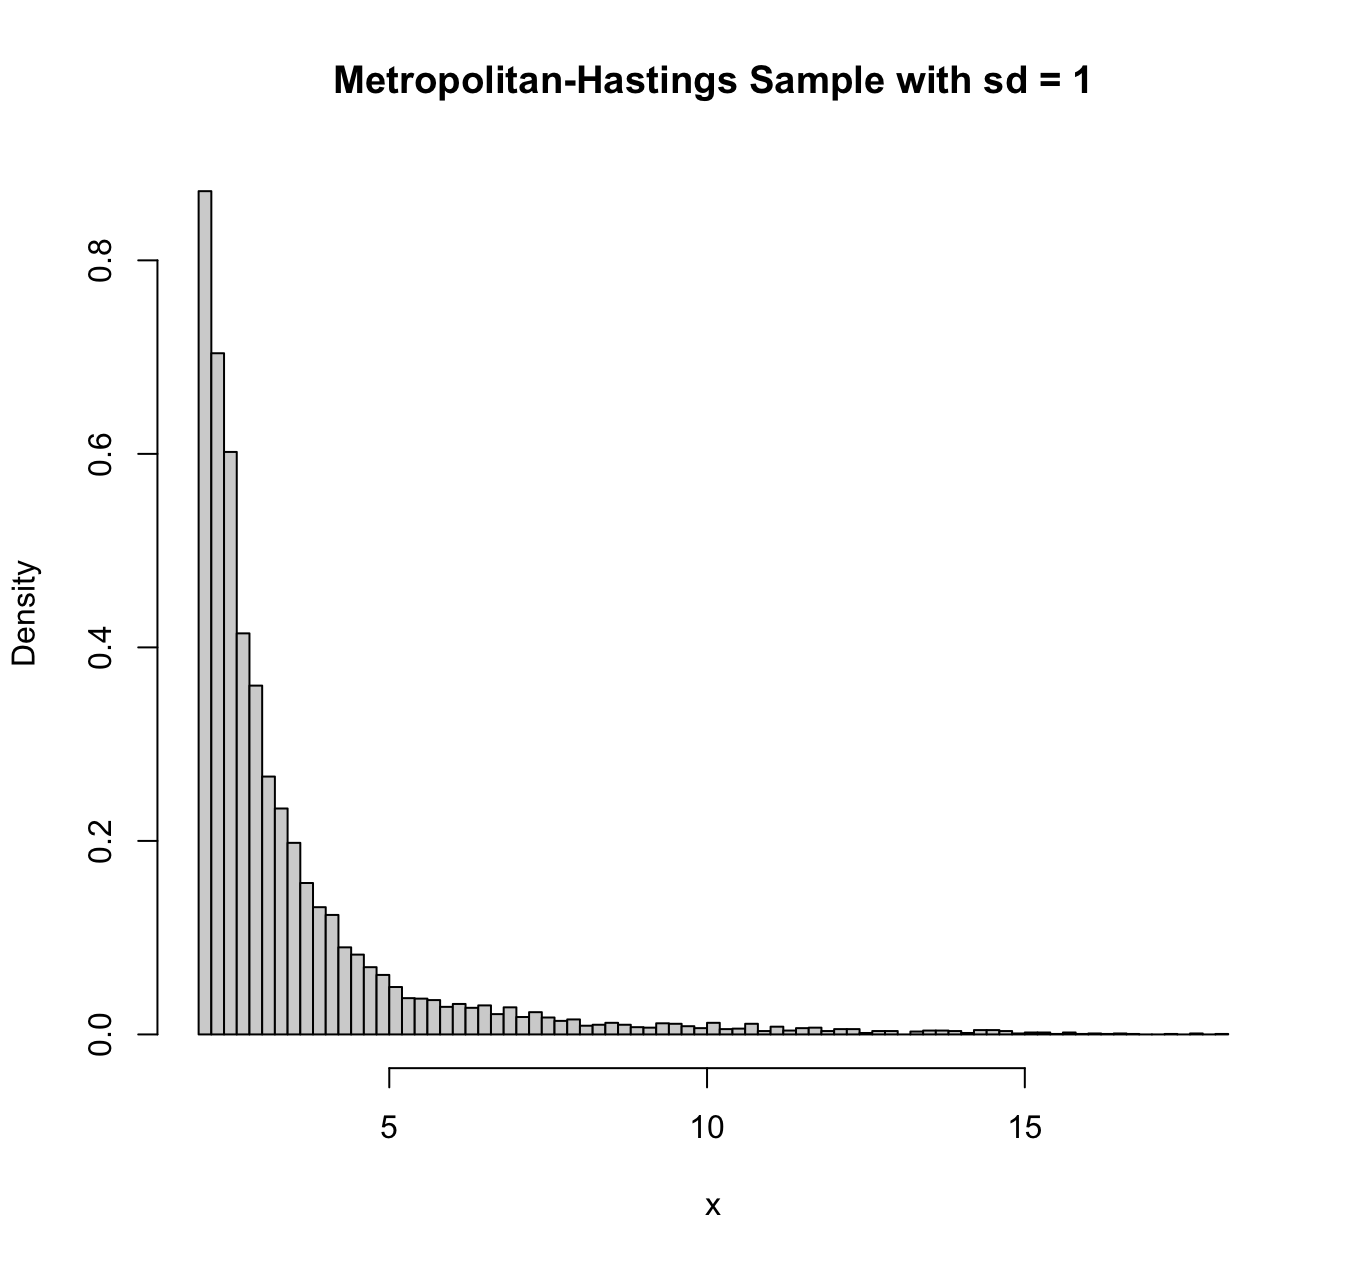
\includegraphics[width=0.65\textwidth]{problem_1_met_hastings_sd_1_hist.png}
\end{figure}
\begin{figure}[H]
    \centering
    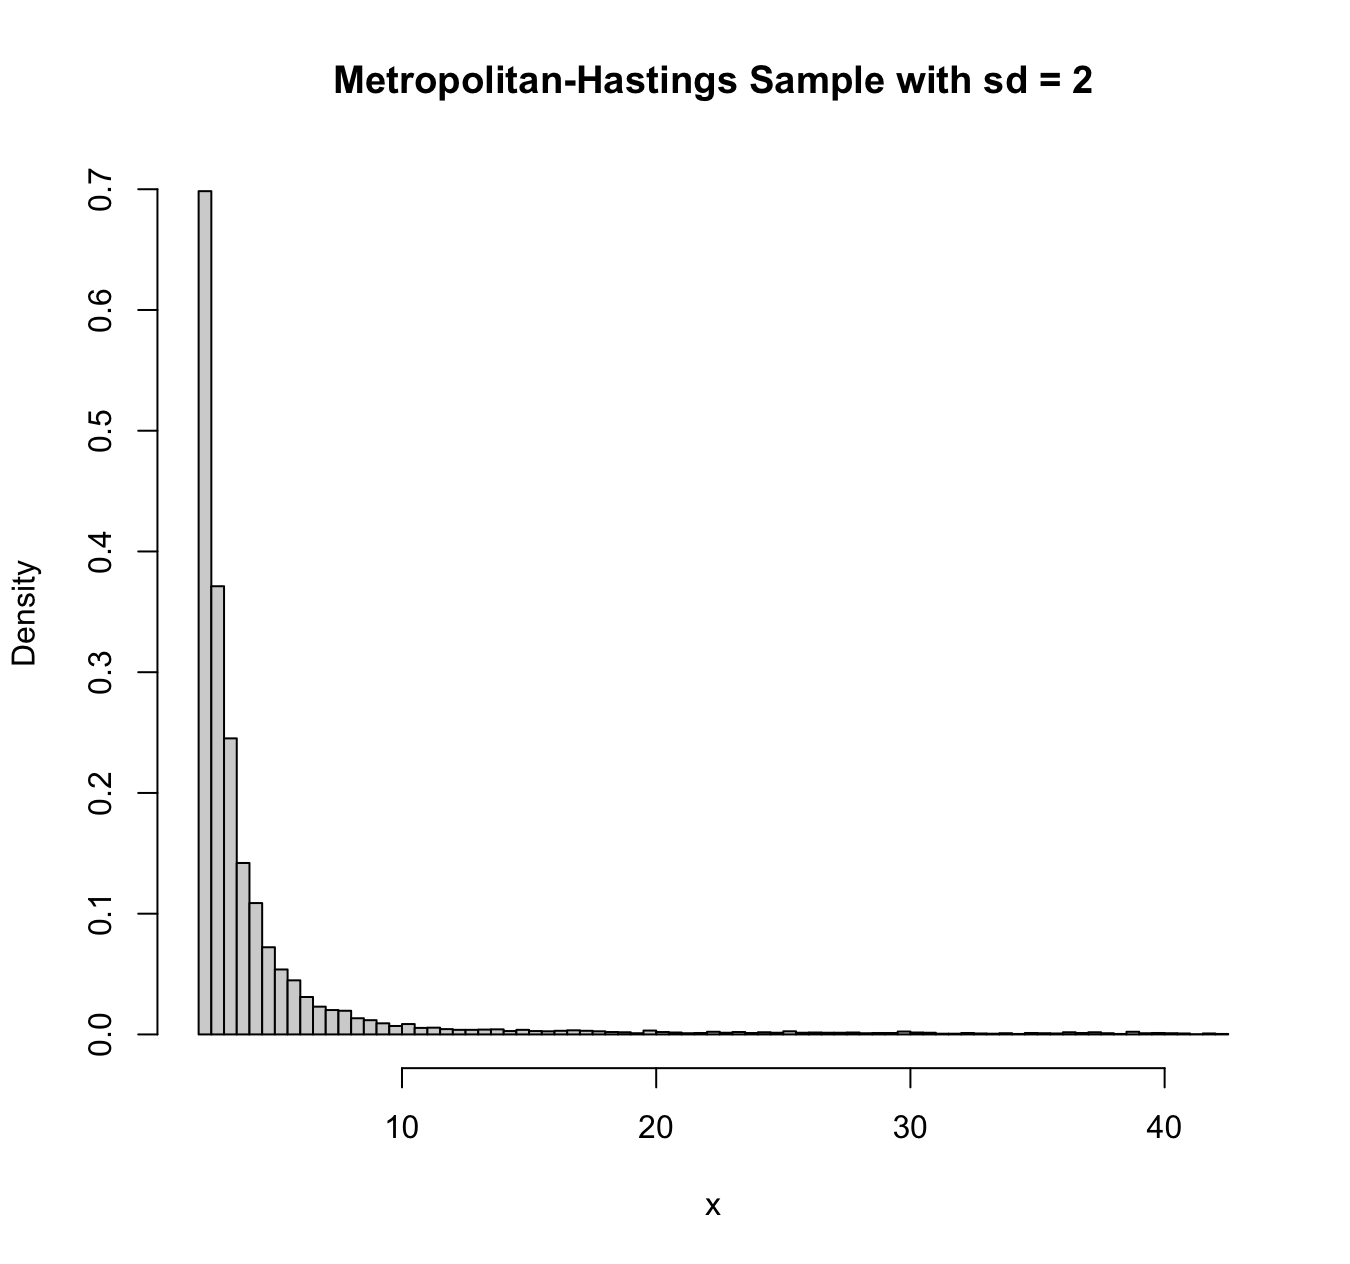
\includegraphics[width=0.65\textwidth]{problem_1_met_hastings_sd_2_hist.png}
\end{figure}
\begin{figure}[H]
    \centering
    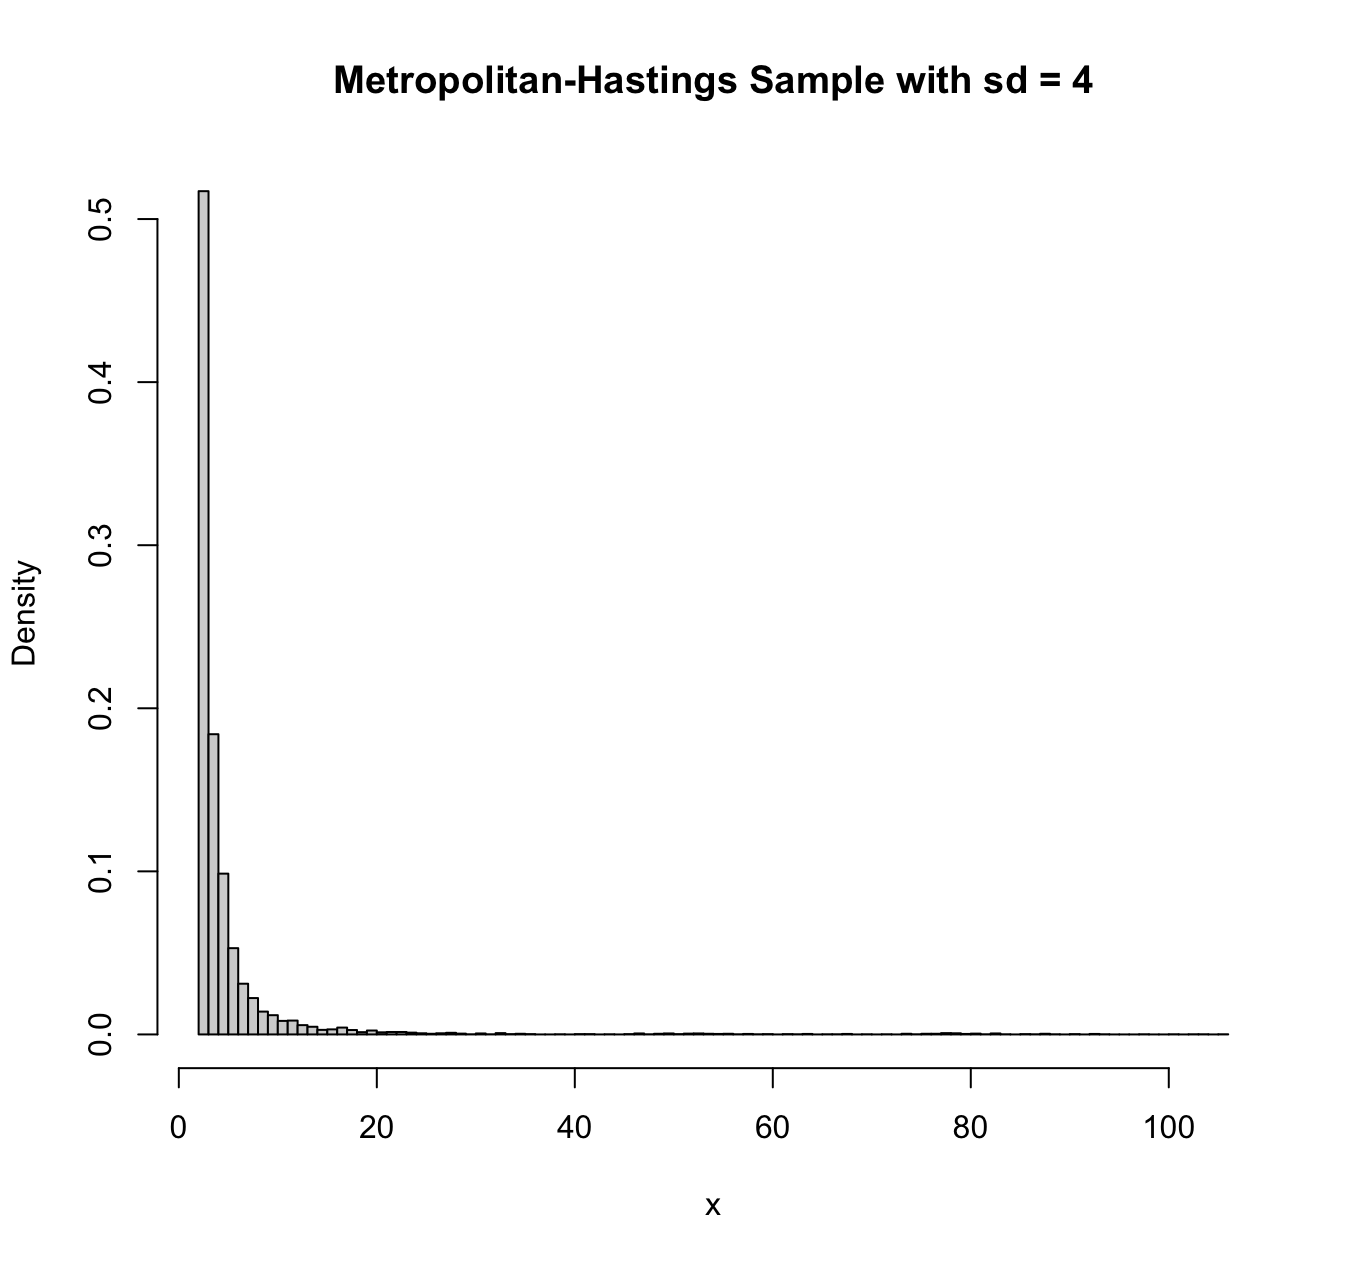
\includegraphics[width=0.65\textwidth]{problem_1_met_hastings_sd_4_hist.png}
\end{figure}

}
{\Large 

\section*{2.}

We are given the random variables \(X\) and \(Y\) which both take on values in the interval \((0, B)\). We are given the following joint densities:
\[
  f(x | y) = C(y)\exp(-xy) \quad 0 < x < B
\]
\[
  f(y | x) = C(x)\exp(-xy) \quad 0 < y < B
\]
where \(C(y)\) is some constant that depends on \(y\) and \(C(x)\) is some constant that depends on \(X\). The provision of both full conditional distributions gives us a hint here, where we intend to simulate values of \(X\) and \(Y\) using the Gibbs Sampling algorithm. We need to find how to sample at each step, though. \\ \\ 
Let's find the constants in terms of \(y\) and \(x\). We need only solve one to find the other, since they are symmetric (i.e. we can swap \(x\) for \(y\) after solving). We can take the CDF and set equal to 1 to solve:
\[
  1 = \int_{0}^{B} C(y) \exp(-xy) dx
\]
\[
  1 = C(y) \frac{e^{-xy}}{-y} |_{0}^{B}
\]
\[
  1 = C(y) (\frac{e^{-By}}{-y} - \frac{e^{0}}{-y})
\]
\[
  1 = C(y) (\frac{1 - e^{-By}}{y})
\]
\[
  C(y) = \frac{y}{1 - e^{-By}}
\]
Now, find the CDF as we normally do:
\[
  F(x|y) = \int_0^x C(y) \exp(-ty) dt
\]
\[
  F(x|y) = C(y) \int_0^x \exp(-ty) dt
\]
\[
  F(x|y) = \frac{y}{1 - e^{-By}} \int_0^x \exp(-ty) dt
\]
\[
  F(x|y) = \frac{y}{1 - e^{-By}} \cdot \frac{e^{-ty}}{-y} |_0^x 
\]
\[
  F(x|y) = \frac{y}{1 - e^{-By}} (\frac{e^{-xy}}{-y} - \frac{e^{0}}{-y})
\]
\[
  F(x|y) = \frac{y}{1 - e^{-By}} (\frac{1 - e^{-xy}}{y})
\]
\[
  F(x|y) = \frac{1 - e^{-xy}}{1 - e^{-By}}
\]
Inverting seems to work well here:
\[
  U = \frac{1 - e^{-xy}}{1 - e^{-By}}
\]
\[
  U(1 - e^{-By}) = 1 - e^{-xy}
\]
\[
  e^{-xy} = 1 - U(1 - e^{-By})
\]
\[
  -xy = \ln(1 - U(1 - e^{-By}))
\]
\[
  x = F^{-1}(U) = -\frac{\ln(1 - U(1 - e^{-By}))}{y}
\]
We can now proceed with our sampling, alternating between getting \(X|Y\) and \(Y|X\). Within each sample, we draw using the inverse transform method. Our sampling algorithm takes the following form now: \\
- Set \(X^0\) and \(Y^0\) to some arbitrary starting value within the range of \((0, B)\) \\
- Generate \(X^{t+1}\) from \(f (x | y) = Y^t\) using the inverse transform method and function we just found; that is, first generate some \(U \sim \text{Unif}(0, 1)\) and set \(X^{t+1} = -\frac{\ln(1 - U(1 - e^{-BY^t}))}{Y^t} \) \\
- Generate \(Y^{t+1}\) from \(f (y | x) = X^{t+1}\) using the inverse transform method and symmetrical version of the function we just found; that is, first generate some new \(U \sim \text{Unif}(0, 1)\) and set \(Y^{t+1} = -\frac{\ln(1 - U(1 - e^{-BX^{t+1}}))}{X^{t+1}} \) \\
- Repeat the above two steps for the desired number of sample pairs, which is our final simulation of \(X\) and \(Y\)

}
{\Large 

\section*{3.}

We aim to estimate the following integral using importance sampling:
\[
  \int_{0}^{\infty} x^2 \sin(\pi x)e^{-\frac{x}{2}}dx
\]
In importance sampling, we sample from a different density that is easier to sample from, and computing the estimate
\[
  \hat{E}[h(X)] = \frac{1}{n} \sum h(X_j) \frac{f(X_j)}{g(X_j)}
\]
A natural choice here for \(g(x)\) is something exponential. It makes more sense to match this dominant decay, which is the exponential term, while sin is hard to sample from effectively and something power-based like \(x^2\) doesn't fit the shape of the function as well and is dominated by the other terms in the integral. The exponential likely cancels out well with the last term as well. Let's try a \(\exp(\lambda) = \lambda e^{-\lambda x}\), which cancels out well with \(\lambda = \frac{1}{2}\). So using \(g(x) = \exp(\frac{1}{2}) = \frac{e^{-\frac{x}{2}}}{2}\):
\[
  \int_{0}^{\infty} x^2 \sin(\pi x)e^{-\frac{x}{2}}dx
\]
\[
  = \int_{0}^{\infty} \frac{x^2 \sin(\pi x)e^{-\frac{x}{2}}}{g(x)} g(x) dx
\]
\[
  = \int_{0}^{\infty} \frac{x^2 \sin(\pi x)e^{-\frac{x}{2}}}{\frac{e^{-\frac{x}{2}}}{2}} \cdot \frac{e^{-\frac{x}{2}}}{2} dx
\]
\[
  = \int_{0}^{\infty} 2x^2 \sin(\pi x) \cdot \frac{e^{-\frac{x}{2}}}{2} dx
\]
\[
  = E_g [2x^2 \sin(\pi x)]
\]
which works out great! We can now approximate this integral by generating values \(X_1, X_2, \dots, X_n\) from our chosen \(g(x)\) and calculate the estimate \(\hat{E}[h(X)]\) as desired above. 

\begin{spverbatim}
> n = 1000
> 
> # h(x) = f(x) / g(x)
> h = function(x) {
+   2 * x^2 * sin(pi * x)
+ }
> 
> importance_sampling = function(n) {
+   # Generate samples from our chosen g(x)
+   x = rexp(n, rate = 1 / 2)
+   
+   # Evaluate h(x) at the sample points
+   h_x = h(x)
+   
+   integral_estimate = mean(h_x)
+   
+   plot(
+     cumsum(h_x) / 1:n,
+     type = "l",
+     xlab = "Number of samples",
+     ylab = "Integral estimate",
+     main = paste(
+       "Importance Sampling Estimate with n =", 
+       n,
+       ", mean =",
+       integral_estimate
+     )
+   )
+   print(paste("Integral estimate:", integral_estimate))
+ }
> 
> importance_sampling(n)
[1] "Integral estimate: -0.506219034838575"
\end{spverbatim}
\begin{figure}[H]
    \centering
    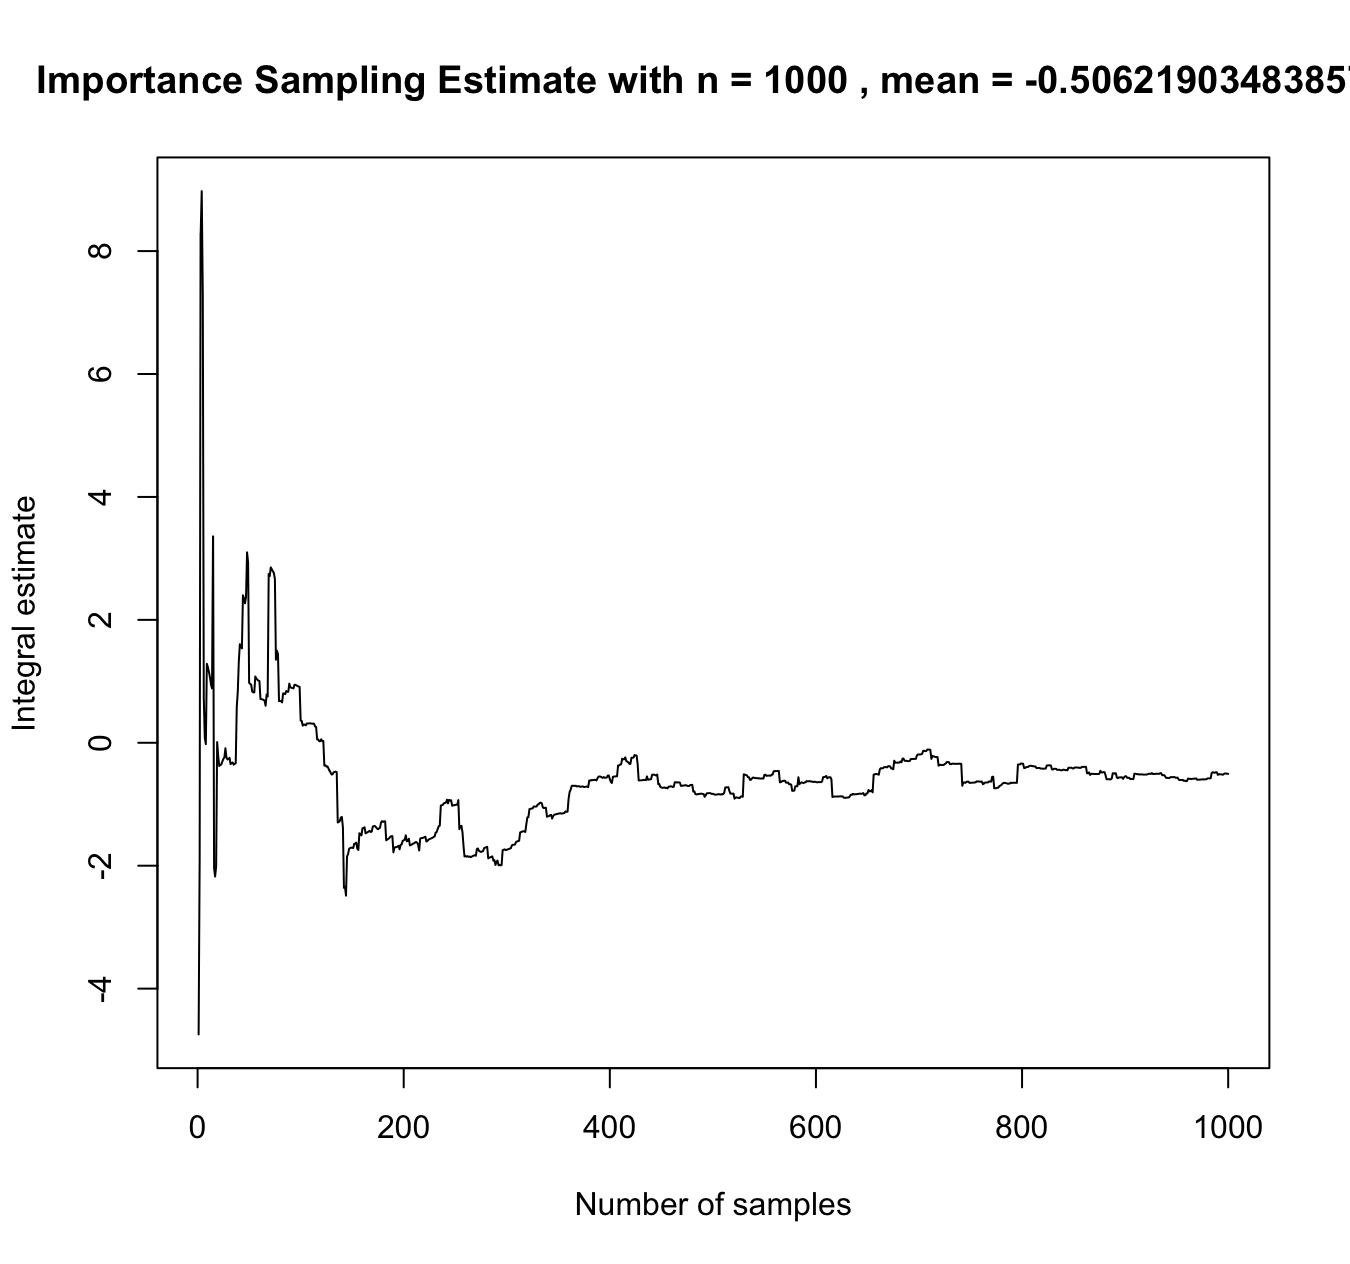
\includegraphics[width=0.8\textwidth]{problem_3_importance_plot.png}
\end{figure}
In this code, we first the function \(h(x) = \frac{f(x)}{g(x)}\) which we've already found above, with these being the values that we compute and take the mean of. We then get to the heart of the importance sampling function. We first sample based on the \(g(x)\) that we picked, and evaluate these values at \(h(x)\) accordingly. We then compute the actual estimate by taking the mean and plot the results, which indicate eventual convergence after some early jumping around. 


}
{\Large 

\section*{4.}

We aim to implement the antithetic variable scheme to see whether it leads to variance reduction when estimating the mean of \(X\), where \(X \sim f_X(x) = 2x^{-3}\) for \(x > 1\). \\ \\
Let's begin with the inverse transform process, first finding the CDF:
\[
  F(x) = \int_1^x \frac{2}{t^3} dt 
\]
\[
  F(x) = -\frac{2}{2t^2} |_1^x 
\]
\[
  F(x) = -\frac{1}{x^2} - (-\frac{1}{1^2})
\]
\[
  F(x) =  1 - \frac{1}{x^2} 
\]
Now inverting:
\[
  U = 1 - \frac{1}{x^2}
\]
\[
  \frac{1}{x^2} = 1 - U
\]
\[
  1 = (1 - U)x^2
\]
\[
  x = \frac{1}{\sqrt{1 - U}}
\]

We can now perform the estimation and compare accordingly. For the antithetic variable scheme: \\ 
- Generate \(U_1, U_2, \dots, U_n \sim \text{Unif}(0, 1)\) \\ 
- Set \(X_j = F_X^{-1}(U_j) = \frac{1}{\sqrt{1 - U}}\) \\
- Set \(Y_j = F_X^{-1}(1 - U_j) = \frac{1}{\sqrt{1 - (1 - U)}}\) \\
- Set \(Y_j = F_X^{-1}(1 - U_j) = \frac{1}{\sqrt{1 - (1 - U)}} = \frac{1}{\sqrt{U}}\) \\
\begin{spverbatim}
> n = 1000
> nmbSimulations = 1000
> 
> antithetic_comparison = function(n, nmbSimulations) {
+   brute_force_means = rep(0, nmbSimulations)
+   antithetic_means = rep(0, nmbSimulations)
+     
+   for (i in 1:nmbSimulations) {
+     # Brute force, simulate using inverse-transform directly
+     U = runif(2 * n)
+     X = 1 / sqrt(1 - U)
+     brute_force_means[i] = mean(X)
+     
+     # Antithetic approach in pairs
+     U = runif(n)
+     X = 1 / sqrt(1 - U)
+     Y = 1 / sqrt(U)
+     antithetic_means[i] = mean((X + Y) / 2)
+   }
+       
+   print(paste("Brute force mean estimate mean:", mean(brute_force_means)))
+   print(paste("Brute force mean estimate variance:", var(brute_force_means)))
+   print(paste("Antithetic mean estimate mean:", mean(antithetic_means)))
+   print(paste("Antithetic mean estimate variance:", var(antithetic_means)))
+   
+   par(mfrow = c(1, 2))
+   hist(brute_force_means, breaks = 60, main = "Brute Force Means")
+   hist(antithetic_means, breaks = 60, main = "Antithetic Means")
+ }
> 
> antithetic_comparison(n, nmbSimulations)
[1] "Brute force mean estimate mean: 2.00222309099802"
[1] "Brute force mean estimate variance: 0.0106837846732948"
[1] "Antithetic mean estimate mean: 2.00169191480643"
[1] "Antithetic mean estimate variance: 0.0054753456242509"
\end{spverbatim}
In the code, we run 1000 simulations for \(n = 1000\). We first simulate 2000 values from the uniform distribution (doubled because we are using the antithetic paired approach later, for which we simulate 10000 values each) and then take the inverse function value directly, and take the mean of these resulting values. This is the brute force approach. For the antithetic method, we take 1000 values from the uniform distribution and then find the corresponding \(X\) and \(Y\) values from the inverse function that we previously found, and then take the mean based off of the resulting 1000 averages of these two paired values, as is described by the antithetic method. We then print the results and plot accordingly. \\ \\ 
We see that both mean estimates for the mean are pretty close to 2, but the variance of them mean estimate with the antithetic method is indeed a bit lower, so there seems to be some variance reduction using the method when estimating the mean of \(X\) in this case.
\begin{figure}[H]
    \centering
    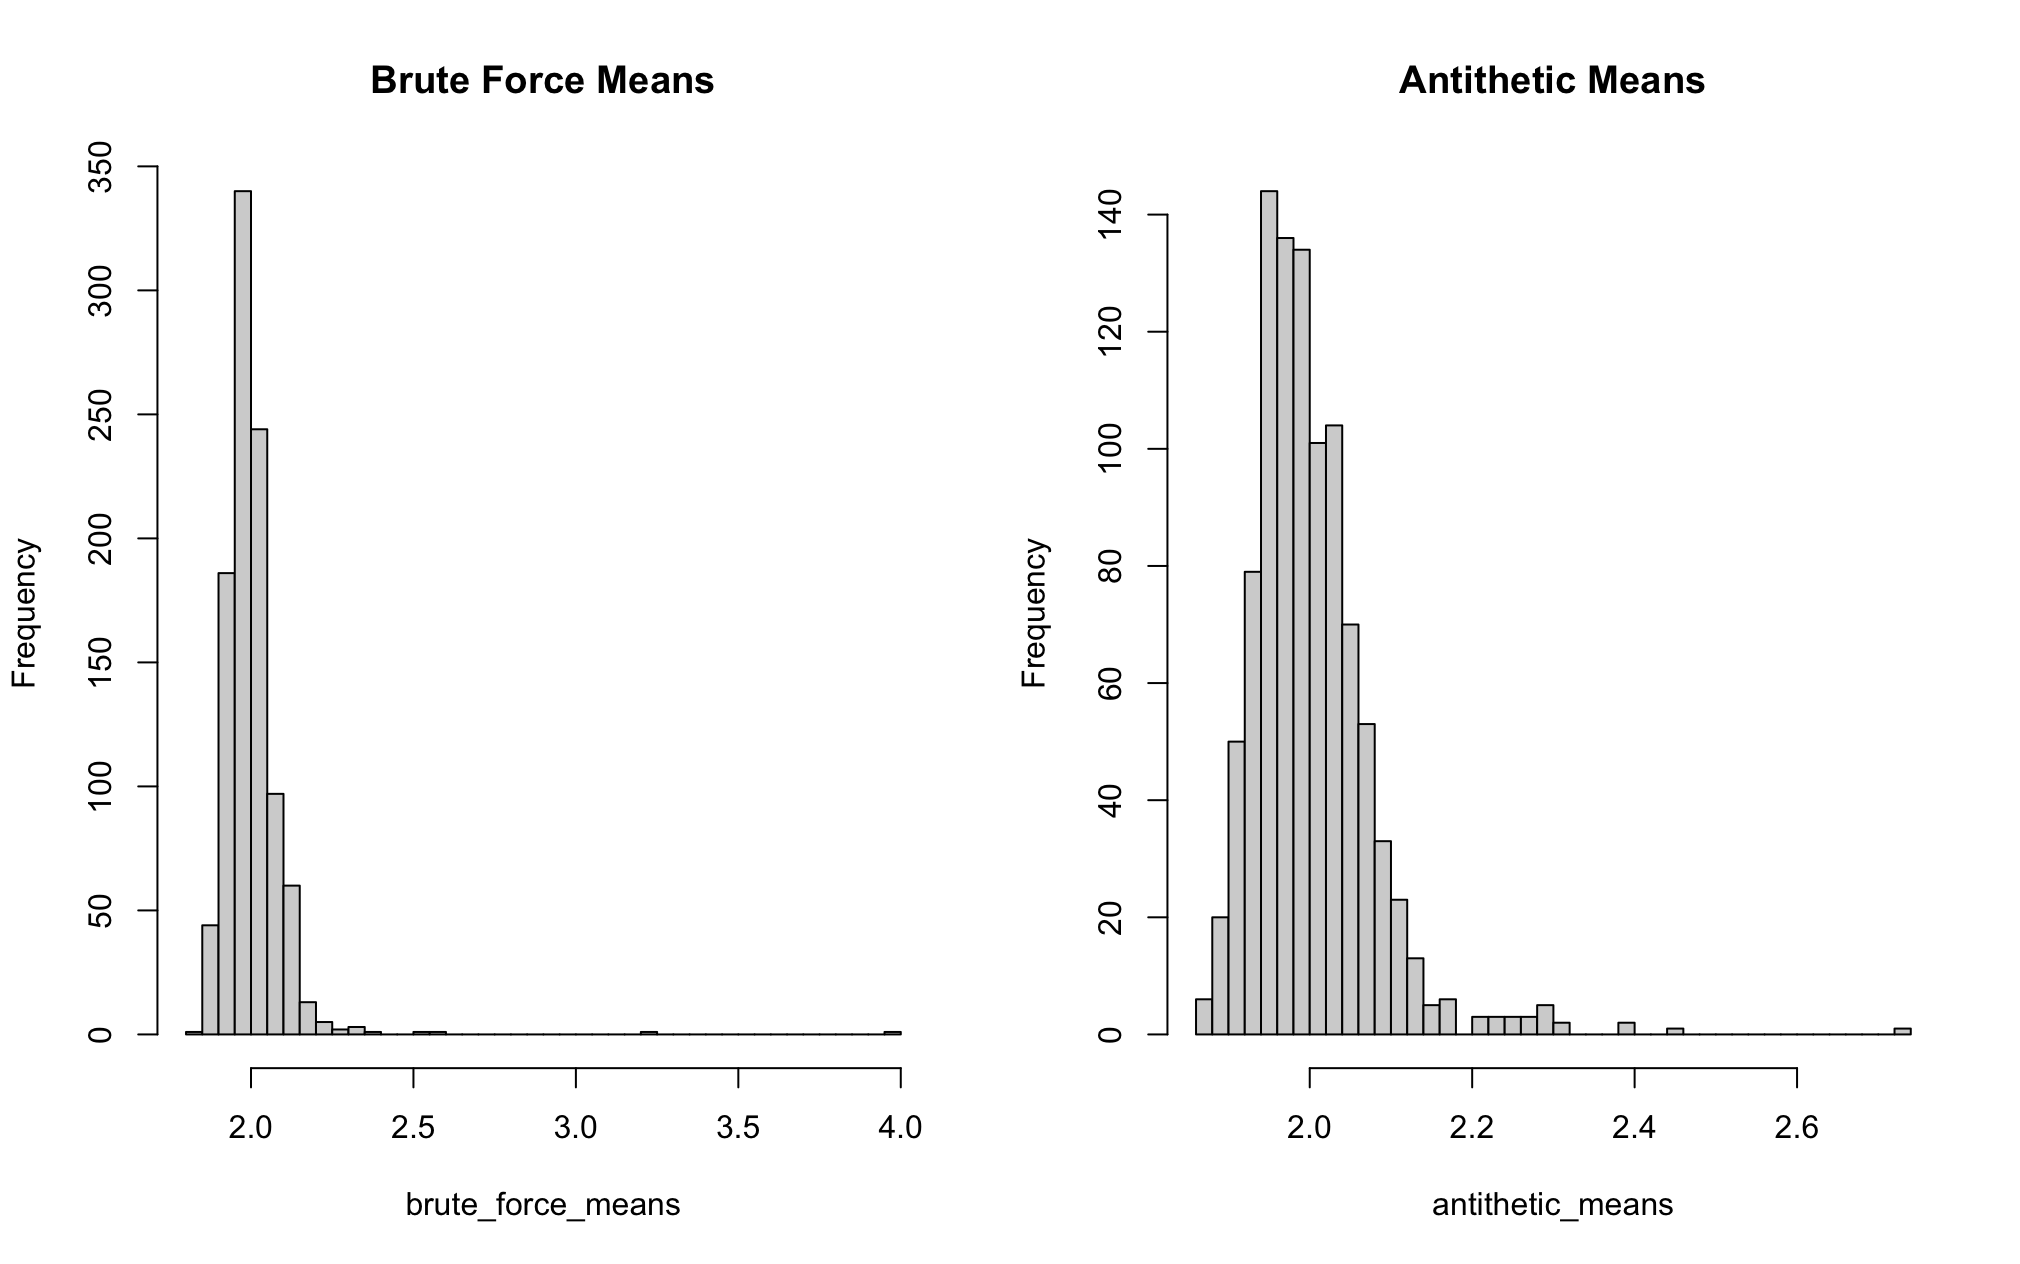
\includegraphics[width=1\textwidth]{problem_4_antithetic_hist.png}
\end{figure}

}
{\Large 

\section*{5.}

Dear Dr. Botts, I have a lot of respect for your commitment to continued learning, especially in a field like statistics. To help out and hopefully tickle your brain a bit, I'd like to explain some useful techniques used in the real world related to estimating simple statistics based on sample data. Normally, we can easily use formulas to estimate confidence intervals of statistics of sample data. However, this doesn't always work -- we need enough data and always assume that the data is normally distributed (i.e. eventually forms the overall shape of a bell curve). While some data samples do fulfill this criteria (or at least often enough for this to be a common idea taught in introductory statistics), this often doesn't work with real-life cases, where you want more complex statistics (like the median or correlations between samples) or often don't have enough samples or aren't able to assume normality of the data in good faith. We therefore can't use these simple formulas based on the normal distribution to determine the error of your target estimate statistics and build a confidence interval around this. We need a better way of quantifying this uncertainty range around performing statistical analyses on a sample in these non-standard, cookie cutter situations. \\ \\
Enter the Bootstrap. We use the Bootstrap to determine the standard error by treating the sample as if it were our actual population, rather than assuming some larger population distribution as we do when using normalized methods. We repeatedly sample the given data with replacement \(n\) times, where the number of data points we are given is \(n\). So we now have a new sample of \(n\) points from our initial data, with the possibility of repetitions given our new. Given this new sample, we then calculate the actual target statistic. We perform this many times to get a good spread of the actual statistic. We then can calculate the confidence interval based on this spread. This is incredibly useful in the way that it essentially works for any kind of statistic, no matter how complex. So for example, given a sample of 10 data points, we create a new sample of size 10 by sampling with replacement from the data points 10 times, and then calculate our target statistic on this new sample. We repeat this an arbitrary amount of times -- say 1000 times -- and then we can calculate the confidence interval based on those 1000 target statistics (e.g. take the middle 95\% from the 2.5 to the 97.5 percentile values to get the 95\% CI, etc.). \\ \\
Now, there are some cases in which it can be impractical or undesirable to do the Bootstrap. Say that it's impractical to compute an arbitrary amount of times (sometimes hundreds to thousands to get meaningful values), or I want to make my results from a sample comparable against other samples without the randomness of sampling with replacement involved. In these kinds of cases, we can use the Jackknife. The Jackknife takes a similar approach, but when we create our new samples, we simply remove one value from the initial given values, and compute the statistic based on the remaining \(n-1\) (also dubbed the "leave-one-out" approach). Intuitively, we can repeat this process only \(n\) times, which is significantly simpler, and notably also non-random compared to the Bootstrap, since we know that we will have a sample in which every single individual value is left out at some point. Intuitively, this also indicates that with a smaller sample size, \(n\) will be much smaller than the arbitrary number of repetitions we need in the Bootstrap, so the Jackknife is also better with smaller samples, with it being less expensive and more convenient as a result. It should be noted, however, that the Jackknife does struggle with statistics that aren't affected as much by just leaving one sample out, such as the median, which can theoretically always stay the same when leaving one sample out -- so there is some discretion needed in choosing between the Bootstrap and the Jackknife. Hope that helps.

}
{\Large 

\section*{6.}

\subsection*{(a)} 

We aim to use the bootstrap method to estimate the probability that a random variable coming from this distribution is less than 0.75, with a 95\% confidence interval. 
\begin{spverbatim}
> data = c(1.491, 0.019, 0.318, 0.056, 0.816, 0.978, 0.174, 0.461, 
+          0.495, 0.547, 0.123, 2.270, 0.026, 0.041, 0.391)
> n = length(data)
> B = 1000
> threshold = 0.75
> 
> bootstrap_prob = function(data, B, threshold) {
+   # Clever way to calculate probability using one-hot encoding
+   bootstrap_estimate = mean(data < threshold)
+   
+   bootstrap_estimates = rep(0, B)
+   for (i in 1:B) {
+     bootstrap_sample = sample(data, n, replace = TRUE)
+     bootstrap_estimates[i] = mean(bootstrap_sample < threshold)
+   }
+   
+   percentile_ci = quantile(bootstrap_estimates, c(0.025, 0.975))
+   
+   print(paste("Bootstrap estimate:", bootstrap_estimate))
+   print(
+     sprintf(
+       "95%% CI for bootstrap estimate: (%f, %f)",
+       percentile_ci[1], 
+       percentile_ci[2]
+     )
+   )
+   
+   hist(
+     bootstrap_estimates,
+     main = paste(
+       "Bootstrap distribution of Probability that RV <",
+       threshold,
+       "with B =",
+       B
+     )
+   )
+   
+   abline(
+     v = bootstrap_estimate,
+     col = "red"
+   )
+ }
> 
> bootstrap_prob(data, B, threshold)
[1] "Bootstrap estimate: 0.733333333333333"
[1] "95% CI for bootstrap estimate: (0.466667, 0.933333)"
\end{spverbatim}
\begin{figure}[H]
    \centering
    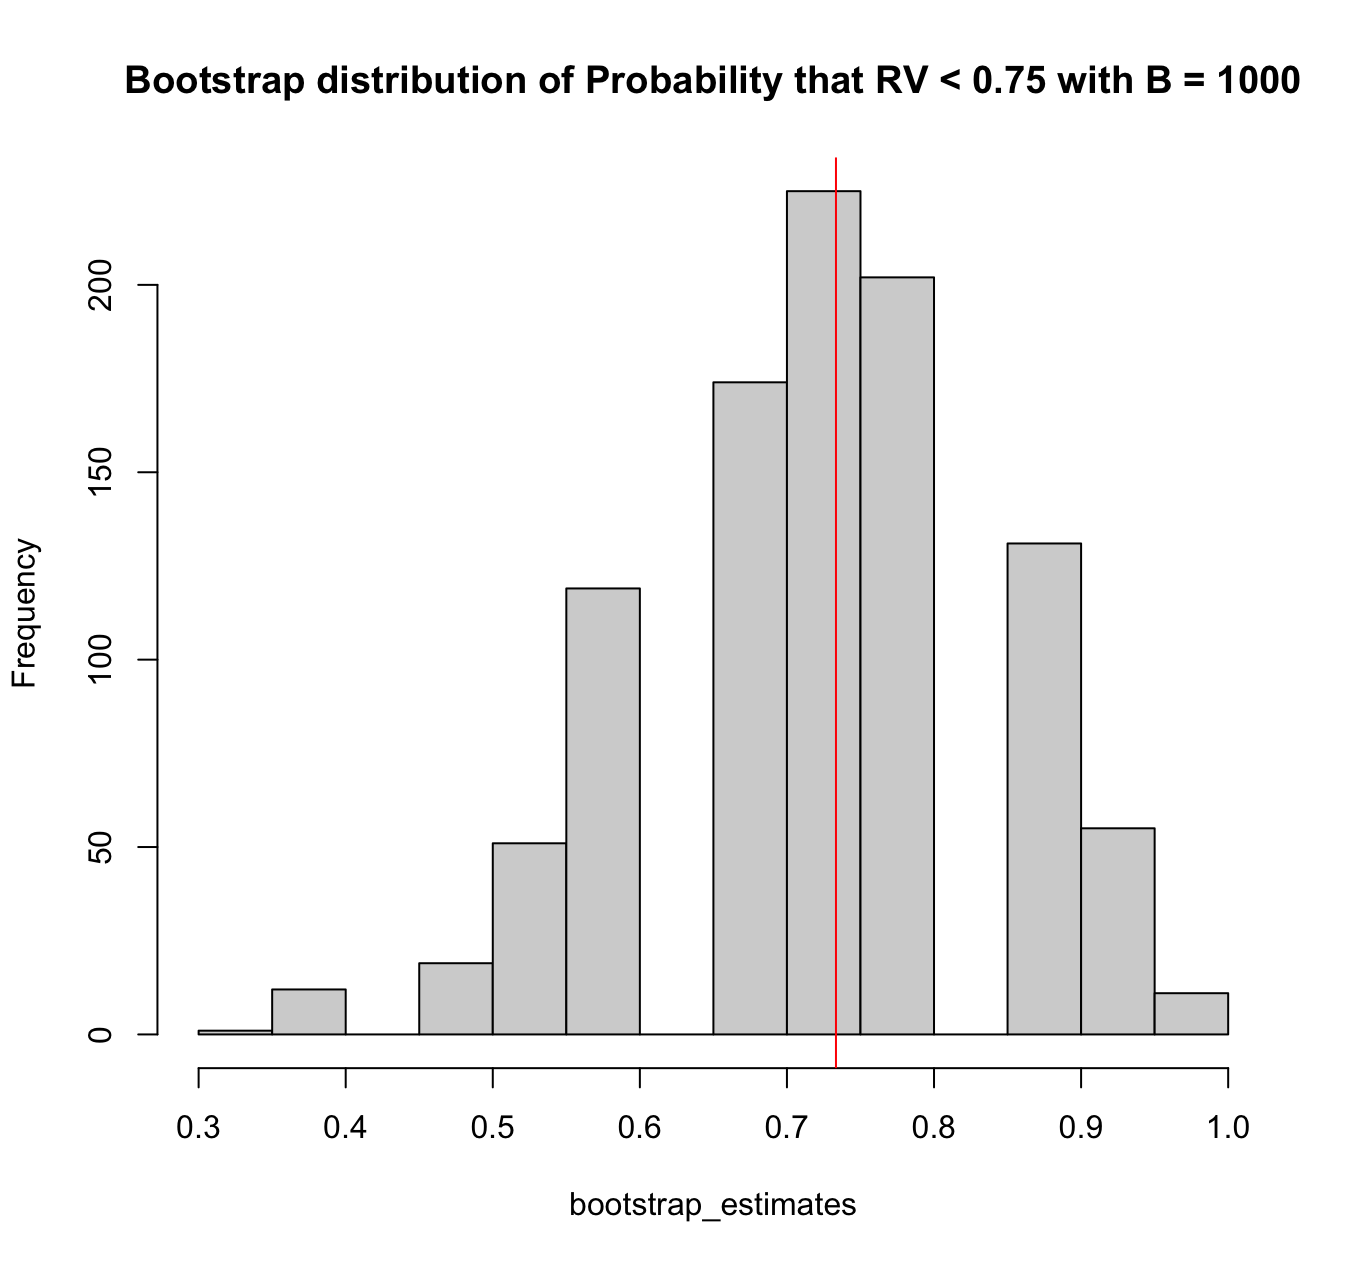
\includegraphics[width=0.75\textwidth]{problem_6_a_bootstrap_hist.png}
\end{figure}
In this code, we first set up the data constants we need for the bootstrap function: the data, the number of data points, the number of bootstrap repetitions, and the threshold for which we want to evalute the probability of the random variables being below. Within the bootstrap function itself, we begin by taking the probability of a random variable being below the given threshold as our original point estimate from the sample data we are provided. We then do the resampling with replacement a arbitrary \(B\) number of times to generate many different samples of size \(n\) for which we take and store their respective probabilities for the random variable being under the threshold. This gives us our actual sample for which we can now calculate the distribution and uncertainty, which we use in this case to calculate the 95\% percentile-based CI between the 2.5\% and 97.5\% percentile of this bootstrapped data. We then print out the estimate and CI alongside a histogram that shows the distribution of the bootstrapped probabilities and the actual estimate point. 

\subsection*{(b)}

Intuitively, it doesn't seem like the bootstrap is a bad choice for performing this estimation: we don't have a great way of determining the actual population distribution, and the number of points is also pretty low, which is a great situation for using the bootstrap. Let's try a study, choosing a super easy known distribution, \(U \sim \text{Unif}(0, 1)\), for which we very intuitively know that \(P(X < 0.75) = \frac{0.75}{1} = 0.75\): 
\begin{spverbatim}
> # Follow up, using Unif(0, 1)
> n = 15
> B = 1000
> threshold = 0.75
> nmbSimulations = 1000
> 
> bootstrap_study = function(n, B, threshold, nmbSimulations) {
+   probability_estimates = rep(0, nmbSimulations)
+   
+   for (i in 1:nmbSimulations) {
+     unif_data = runif(n, 0, 1)
+     
+     bootstrap_estimates = rep(0, B)
+     for (j in 1:B) {
+       bootstrap_sample = sample(unif_data, n, replace = TRUE)
+       bootstrap_estimates[j] = mean(bootstrap_sample < threshold)
+     }
+     
+     probability_estimates[i] = mean(bootstrap_estimates)
+   }
+   
+   true_probability = threshold / 1
+   simulated_probability = mean(probability_estimates)
+   
+   print(paste("True probability:", true_probability))
+   print(paste("Average bootstrap probability estimate:", simulated_probability))
+   print(paste("Diff:", true_probability - simulated_probability))
+   
+   hist(
+     probability_estimates,
+     main = paste(
+       "Bootstrap distribution of P( RV <",
+       threshold,
+       ") with B =",
+       B,
+       "for Unif(0,1)"
+     )
+   )
+   
+   abline(
+     v = true_probability,
+     col = "red"
+   )
+ }
> 
> bootstrap_study(n, B, threshold, nmbSimulations)
[1] "True probability: 0.75"
[1] "Average bootstrap probability estimate: 0.7454742"
[1] "Diff: 0.00452580000000002"
\end{spverbatim}
In this code, we do similar things to the previous bootstrap code by initializing the corresponding bootstrap variables. However, we add \(nmbSimulations\) in order to do a more conclusive study over multiple trials of how the bootstrap behaves. We then write a function that creates an empty array for storing these probability estimate trials and begin running these 1000 trials. Within each trial, we generate \(n = 15\) data points on the \(\text{Unif}(0,1)\) distribution, as the original data also had 15 data points, and then perform the original bootstrap process with the 15-point sampling with replacement 1000 times, each time taking the sample's respective probability of points being below the 0.75 threshold. We then store this result in our greater simulation array. We finally print out the calculated theoretical probability based on our selected uniform distribution and the average simlated probability estimate from our bootstrap simulations and print out the difference and plot the actual distribution alongside the true theoretical probability.
\begin{figure}[H]
    \centering
    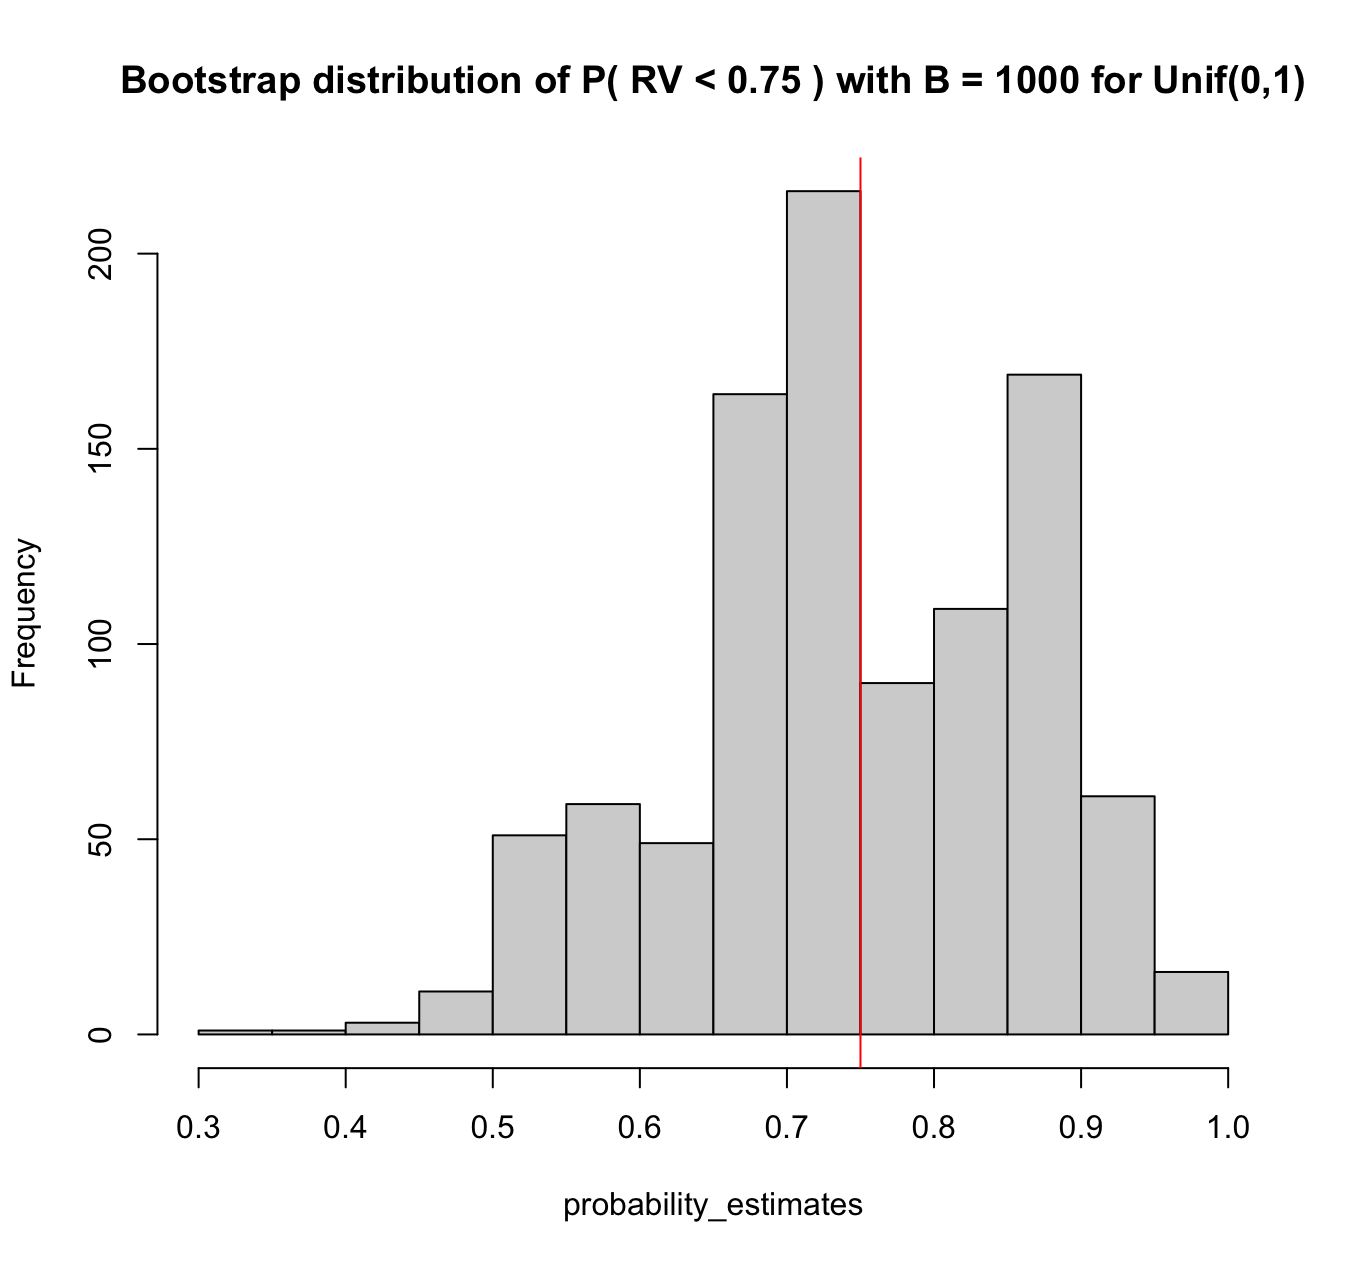
\includegraphics[width=0.75\textwidth]{problem_6_b_bootstrap_study_hist.png}
\end{figure}
The results seem to indicate that the bootstrap really isn't such a bad choice -- the probability difference between the average simulated estimates compared to the theoretical value is actually very small. The results seem to back up the theory pretty well, and the values seem to center pretty well visually on the histogram as well. I'd definitely note that the confidence intervals are pretty wide and suboptimal, but this is more of a product of the low number of points leading to a wider range relative to the overall distribution, which is also magnified by the usage of a 95\% CI which will end up covering a large amount of the range relative to the actual point distribution. 

}
{\Large 

\section*{7.}

Given the stochastic differential equation
\[
  dX(t) = f[X(t)]dt + g[X(t)]dW(t)
\]
The Euler-Maruyama solution to the equation is to set up the discretization as follows: \\ \\ 
- With \(dW_k \sim N(0, \text{Var} = \delta t)\), set up \(W_0 = 0\), \(\delta t = T / N\), \(W_{k+1} = W_k + dW_k\).
- Then, generate the corresponding values \(X_j\) as follows:
\[
  X_j = X_{j-1} + f(X_{j-1})\delta t + g(X_{j-1})dW_k
\]
Dear Dr. Botts, I'm glad that you're continuing your journey in statistics. To help out with this question in particular, we are solving the SDE which represents the change over time of a specific value that we are trying to measure, for example the temperature of a city over time. In the given SDE, we have a more predictable component (the \(f\)) and a more random noise-like component (the \(g\)). For example, we have more predictable components around the seasonality and how we'd expect the temperature to trend as we tilt away/towards the sun, but there is some randomness within the environment that we can't precisely account for/measure (think random bouts of pressure, man-made factors, COVID, natural disasters). \\ \\
Calculating this temperature value over time becomes extremely difficult to model neatly in a simple one-line equation of any form, so we instead use this numerical method called the Euler-Maruyama method which methodically steps through the overall time interval for which we are observing temperature values, chopping this time interval into many different subsections. We represent the width of each time interval in the equation as \(\delta t = T / N\). At each subsection between times \(j-1\) and \(j\), we take the value of the predictable component \(f\) at \(j-1\), i.e. the beginning of the time subsection. We do the same for the random noise function \(g\), but multiply this by a randomly drawn value from a bell curve / normal distribution to represent a randomized added amount of noise. These represent the 2nd and 3rd terms in the equation. We then add both of those values to the final value at the previous time, which is the 1st term in the equation. \\ \\
To make this concrete, we go through each time window; at each time window we would predict the next time window's temperature by summing up the following: the previous time window's temperature, the expected/predictable temperature change based on the seasonality at that given time proportionalized to the width of the time window we are evaluating at, and then the random noise function multiplied by some randomly drawn value from a bell curve / normal distribution. Given that we can't do the actual calculus needed which is very difficult to solve and essentially impossible to directly evaluate in one simple equation, the Euler-Maruyama method "makes sense" because the method faithfully represents the SDE by adding up the constant change and randomized noise at each step proportionalized to each time window size. 

}

\end{document}